\section{Performance Evaluation}
\label{sec:evaluation}

\subsection{Experimental Setup}
\textbf{System Parameters Setup:}
We implement the system in a small scale setting where fully-accessible APs and edge servers are considered.
specifically, there are $K=8$ APs, $M=5$ edge servers, and $J=5$ type of jobs in the system corresponding to the manipulated data trace.
Each time slot is taken as $\tau = 0.05$ i.e. 50ms, and the broadcast interval is taken as $20$ time slots, i.e. $1$ second.
The maximum uploading time is set as $3$ times the broadcast interval, i.e. $\Xi = 3T$.
The distributions of arrival rate, uploading time and processing time are generated randomly.
Each queue for VMs on edge server is set with maximum queue length $L_{max}=20$.
% The arrival rate is taken as small probability with enough APs in the system, and correspondingly enough edge servers for the processing.
% Each queue on edge server with maximum 20 jobs because our algorithm is strong enough to predict the overflow to ensure a reliable system.

\textbf{Compared Algorithms:}
We compare the proposed algorithm with other three heuristic algorithms.
Compared Algorithm:
\begin{itemize}
    \item \textbf{Random Dispatching Policy}:
            randomly dispatch jobs to edge servers;
    \item \textbf{Local Selfish Algorithm (baseline policy)}:
            always choose the edge server with the minimum expected uploading time plus the expected processing time for each job type; this policy is also taken as the initial fixed policy of our proposed algorithm;
    \item \textbf{Local Queue-aware Greedy Algorithm}:
            always choose the edge server with the minimum expected uploading time, plus the expected queueing time based on the observation of stale queue state.
\end{itemize}
Specifically, we choose a heuristic selfish policy as the start and the definition is given as follows.
\begin{definition}[Selfish Policy]
    \begin{align}
        \Baseline &\define \Bracket{ \Pi_{1}, \dots, \Pi_{K} }
        \\
        \pi_{k,j} &\define \arg\min_{m} \mathbb{E}[U_{k,m,j}] + \mathbb{E}[C_{m,j}]
    \end{align} 
\end{definition}
%----------------------------------------------------------------------------------------%

\subsection{Performance Analysis}
    \subsubsection{Basic Performance}
    Here we measure some basic metrics concerning in edge computing system, compared with different algorithms.
    \begin{itemize}
        \item Bar graph: Cost v.s. Algorithms;
        \item Bar graph: JCT v.s. Algorithms;
        \item Bar graph: Total Departure Rate v.s. Algorithms. 
    \end{itemize}

    \subsubsection{Fine-grained Analysis}
    \begin{itemize}
        \item Timeline graph: our proposed algorithm is better than compared algorithms all the time in Fig.\ref{fig:general_timeline};
        \item CDF of Cost (with different algorithms);
        \item CDF of JCT (with different algorithms);
    \end{itemize}

    \subsubsection{Sensitivity Study}
    \begin{itemize}
        \item \textbf{Different number of APs.} (a.k.a arrival rate)
        \item \textbf{Uploading time domains/Processing time domains.}
        \item \textbf{Compared with different \brlatency.} Fig.\ref{fig:eval_delay}
        \item \textbf{Different $t_B$ setting.}
        \item \textbf{Different Penalty Factors.}
    \end{itemize}
    % CDF of \# of dropped jobs (over the queue limit); CDF of queue length;
%----------------------------------------------------------------------------------------%

\begin{figure*}[htp!]
    \centering
    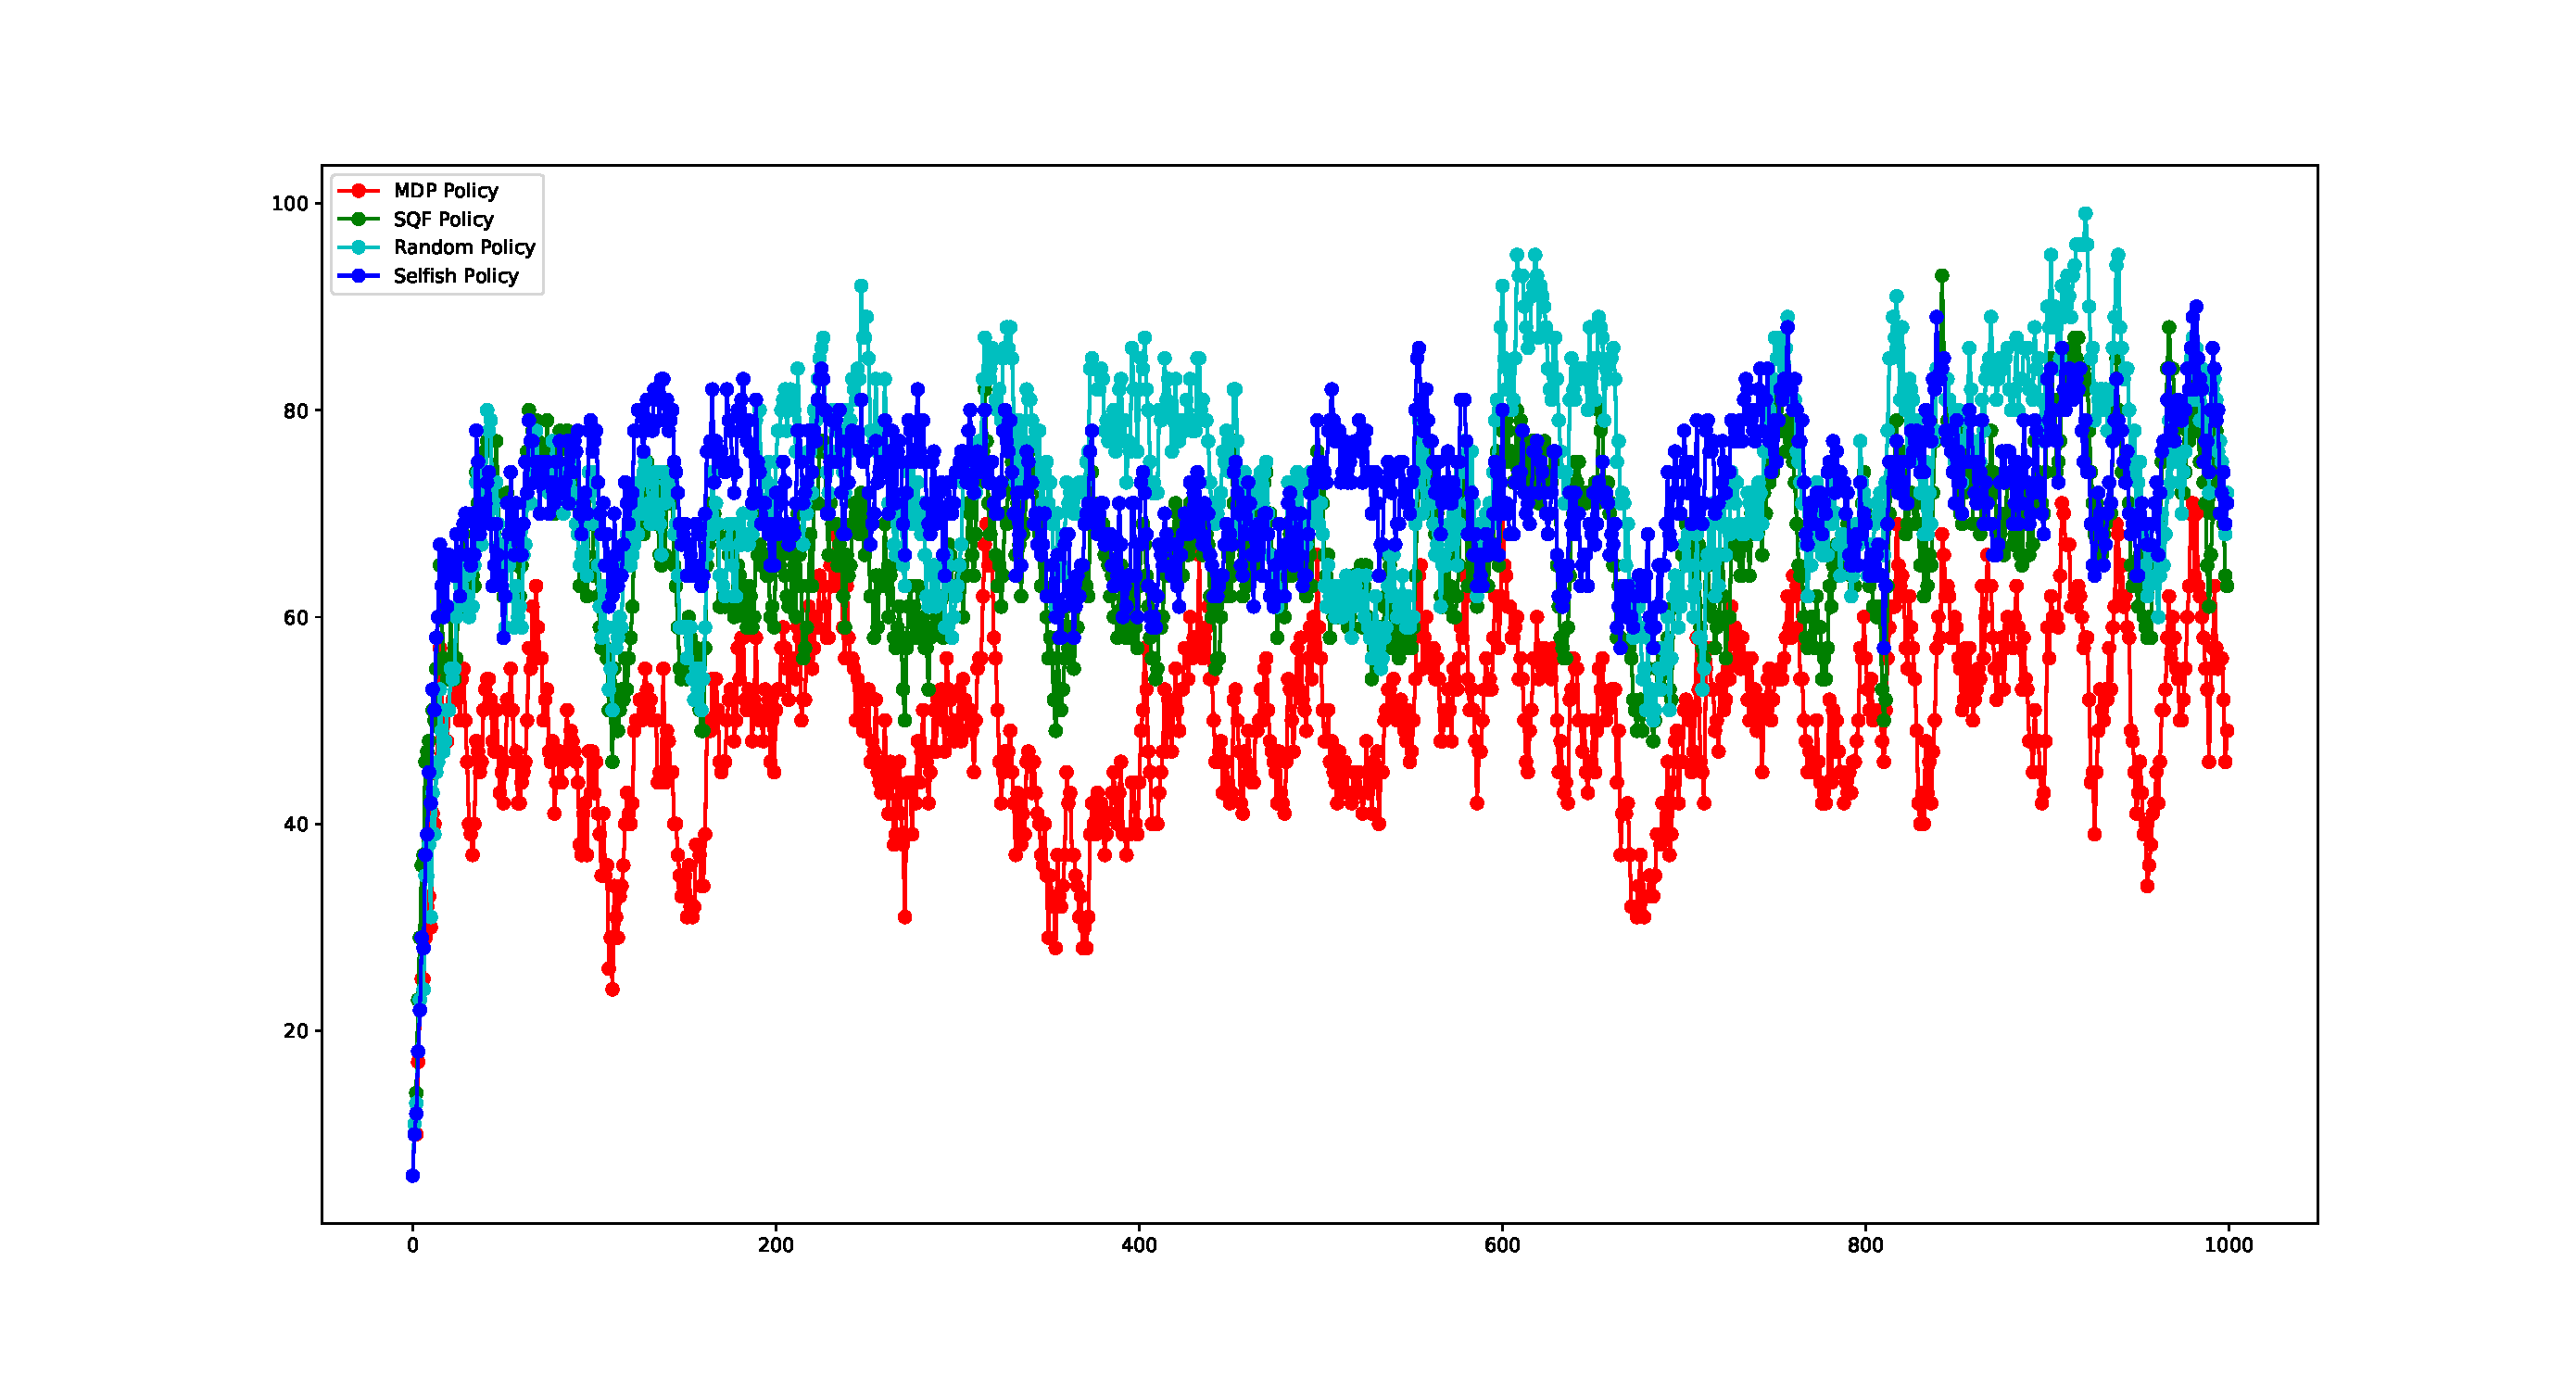
\includegraphics[width=0.80\textwidth]{images/Figure_1.pdf}
    \caption{Timeline illustration.}
    \label{fig:general_timeline}
\end{figure*}

\begin{figure*}[htp!]
    \centering
    \begin{tabular}{ccc}
        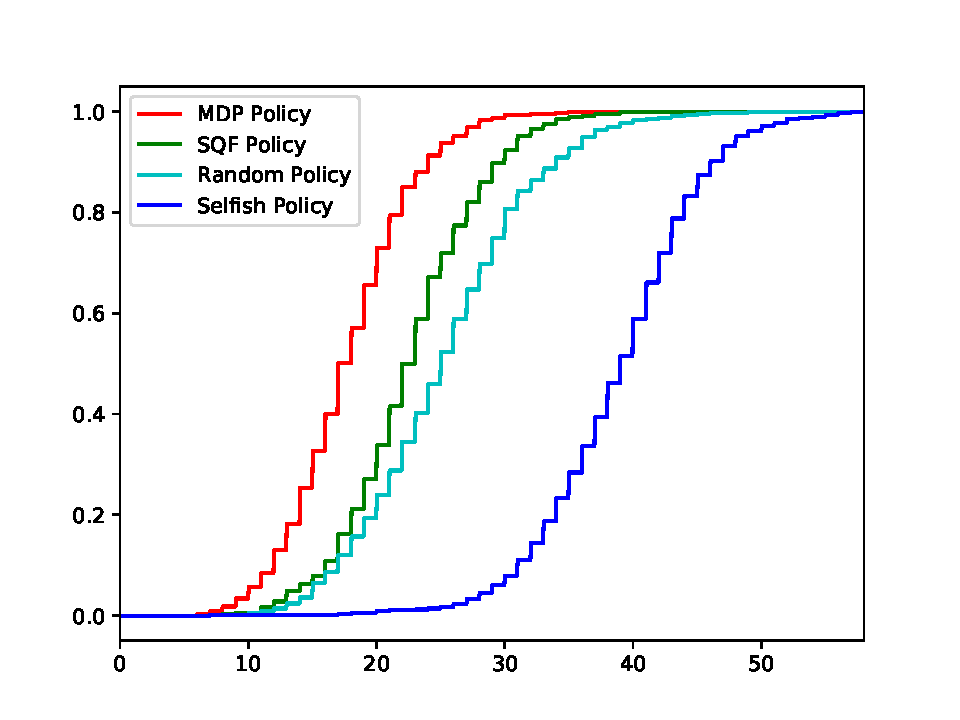
\includegraphics[width=0.30\textwidth]{images/535_LowPressure_NoDelay.pdf}&
        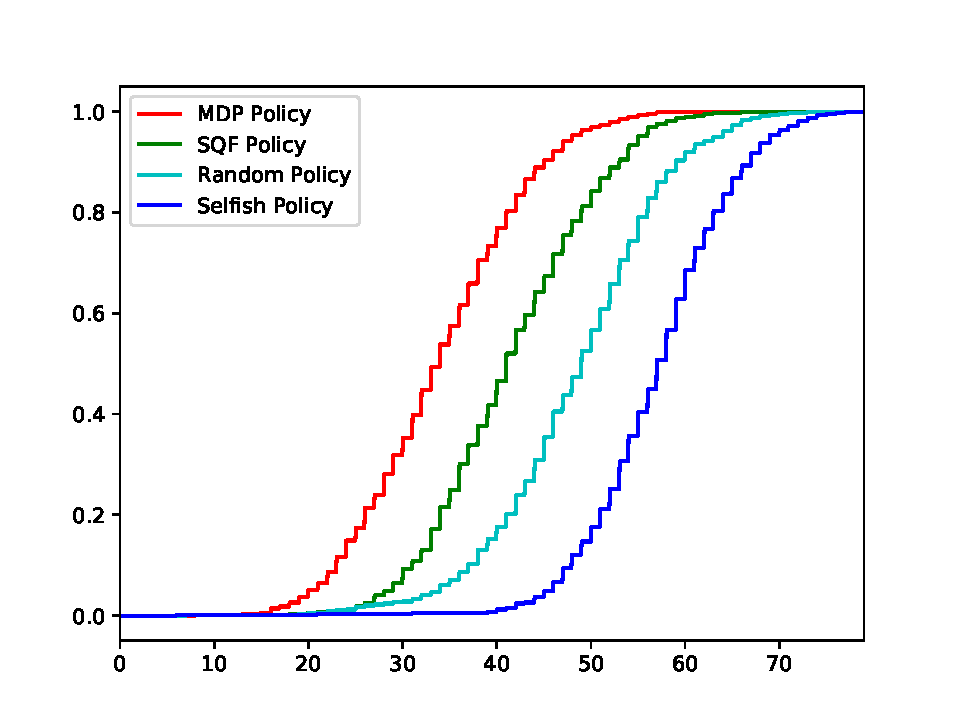
\includegraphics[width=0.30\textwidth]{images/535_LowPressure_LargeDelay_cdf.pdf}&
        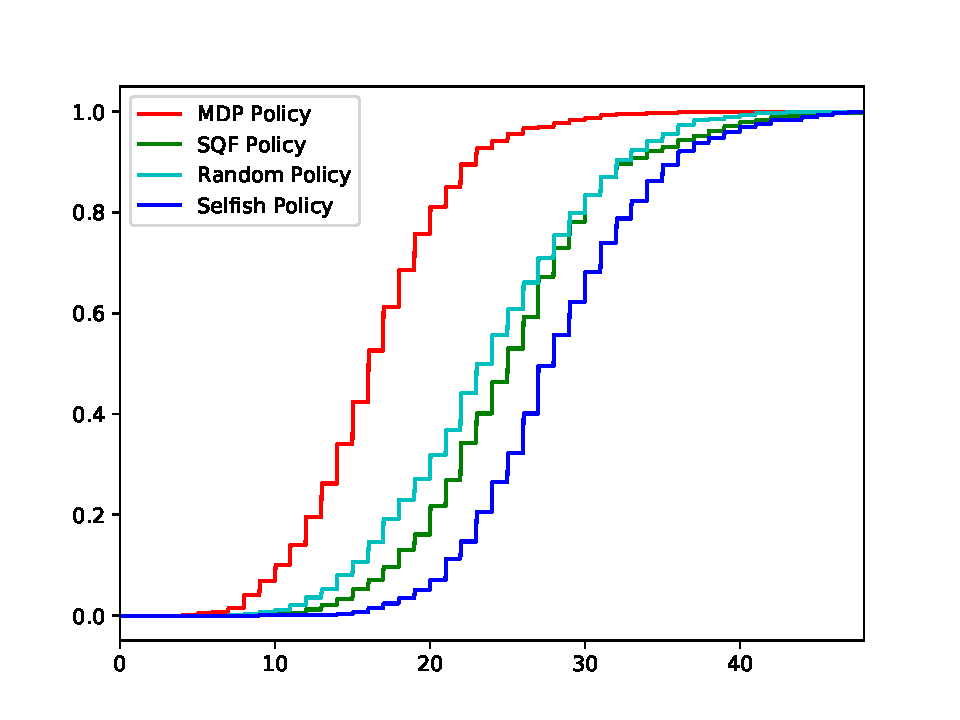
\includegraphics[width=0.30\textwidth]{images/535_LowPressure_FullDelay.pdf}
        \\
        {\small (a) No \brlatency} &
        {\small (b) Large \brlatency} &
        {\small (c) Whole-interval \brlatency}
    \end{tabular}
    \caption{Evaluation of Information Staleness Impact on Algorithm Robustness under Low Back Pressure.}
    \label{fig:eval_delay}
\end{figure*}

\delete{v12.2}{
    \textbf{Data Trace Extraction:}
    We use the Google data trace for cloud computing\needref{google-data-trace}.
    There is no broadcast latency, uploading time, and processing distribution information specified in the data trace.
    Hence, we extract and scale the arrival and processing time in the original data trace.
    And we manipulate the original data with random generated latency distribution.

    % [abandon, cause useless]
    \textbf{Estimation Error Analysis.}
    (If these graphs are not good, they are not going to appear on final draft.)
    \begin{itemize}
        \item Two curves, one for real cost against time slot, one for expected sampling cost against time intervals; (if the accumulate area within the latter one has little/bounded error with real cost, then it is okay and the correctness is support by simulation)
        \item 
    \end{itemize}
}